\documentclass[aspectratio=169,11pt]{beamer}

% ==========================================================
% PACKAGES AND FONTS
% ==========================================================

\usepackage{iftex}

\ifPDFTeX
  \usepackage[T1]{fontenc}
  \usepackage{tgheros}
  \renewcommand{\familydefault}{\sfdefault}
\else
  \usepackage{fontspec}
  \setsansfont{TeX Gyre Heros}
\fi

\usepackage{graphicx}
\usepackage{booktabs}
\usepackage{tabularx}
\usepackage{ragged2e}
\usepackage{tikz}

% ==========================================================
% FIGURE FILES
% ==========================================================

\newcommand{\FigLandscape}{fwa.png}
\newcommand{\FigSetup}{employee_fwa_setup.png}
\newcommand{\FigAwareness}{fwa_awareness.png}
\newcommand{\FigRequests}{formal_requests_outcomes.png}

\newcommand{\FigDCEExample}{dce_example.png}
\newcommand{\FigEmployeeWTP}{employee_wtp_main.png}
\newcommand{\FigEmployerWTP}{employer_wtp_main.png}
\newcommand{\FigGap}{wtp_gap_employee_employer.png}

\newcommand{\FigGenderRemote}{employee_gender_remote.png}
\newcommand{\FigAgeSchedule}{employee_age_schedule.png}

\newcommand{\FigPresence}{employer_physical.png}
\newcommand{\FigConcerns}{employer_concern.png}

\newcommand{\FigEmployeePractice}{employee_current_selected.png}
\newcommand{\FigEmployerPractice}{employer_current_wfh.png}

\newcommand{\StudyName}{SMU--SNEF FWA Study}
\newcommand{\PolicyShare}{66.0}

% ==========================================================
% COLOURS
% ==========================================================

\definecolor{Navy}{HTML}{304A75}
\definecolor{Employee}{HTML}{6D82A0}
\definecolor{EmployeeLight}{HTML}{BED7ED}
\definecolor{Employer}{HTML}{B57A50}
\definecolor{EmployerLight}{HTML}{F2D8B8}

\definecolor{Ink}{HTML}{252B33}
\definecolor{Muted}{HTML}{636B75}
\definecolor{Rule}{HTML}{DFE3E8}
\definecolor{Soft}{HTML}{F5F7FA}

% ==========================================================
% BEAMER STYLE
% ==========================================================

\usetheme{default}

\setbeamertemplate{navigation symbols}{}
\setbeamertemplate{headline}{}

\setbeamercolor{normal text}{fg=Ink,bg=white}
\setbeamercolor{frametitle}{fg=Navy,bg=white}
\setbeamercolor{structure}{fg=Navy}
\setbeamercolor{itemize item}{fg=Navy}
\setbeamercolor{enumerate item}{fg=Navy}

\setbeamersize{
  text margin left=0.65cm,
  text margin right=0.65cm
}

\setbeamerfont{frametitle}{
  size=\fontsize{18}{21}\selectfont,
  series=\bfseries
}

\setbeamerfont{itemize/enumerate body}{
  size=\fontsize{12}{15}\selectfont
}

\setbeamertemplate{itemize item}{\small$\bullet$}

% ==========================================================
% FOOTER
% ==========================================================

\newif\ifappendixslides
\appendixslidesfalse

\newcounter{mainend}

\newcommand{\StartAppendix}{%
  \setcounter{mainend}{\value{framenumber}}%
  \global\appendixslidestrue
}

\newcommand{\DisplayPage}{%
  \ifappendixslides
    A\the\numexpr\value{framenumber}-\value{mainend}\relax
  \else
    \insertframenumber
  \fi
}

\setbeamertemplate{footline}{%
  \leavevmode%
  \hbox{%
    \begin{beamercolorbox}[
      wd=\paperwidth,
      ht=0.25cm,
      dp=0.12cm,
      leftskip=0.65cm,
      rightskip=0.65cm
    ]{normal text}%
      \color{Muted}%
      \fontsize{7.5}{9}\selectfont
      \StudyName
      \ifappendixslides\enspace|\enspace Appendix\fi
      \hfill
      \DisplayPage
    \end{beamercolorbox}%
  }%
}

% ==========================================================
% TEXT ELEMENTS
% ==========================================================

\newcommand{\PanelTitle}[2]{%
  {\color{#1}\fontsize{12.5}{15}\selectfont
   \bfseries #2\par}
  \vspace{0.06cm}
}

\newcommand{\Subline}[1]{%
  {\color{Muted}\fontsize{10}{12.5}\selectfont
   \RaggedRight #1\par}
  \vspace{0.10cm}
}

\newcommand{\SlideNote}[1]{%
  \par\vspace{0.07cm}
  {\color{Muted}\fontsize{7.5}{9}\selectfont
   \RaggedRight #1\par}
}

\newcommand{\Takeaway}[1]{%
  \par\vspace{0.08cm}
  {\color{Rule}\hrule height 0.5pt}
  \vspace{0.08cm}
  {\color{Navy}\fontsize{11}{13.5}\selectfont\bfseries
   \hyphenpenalty=10000\exhyphenpenalty=10000
   \raggedright #1\par}
}

\newcommand{\EditText}[1]{%
  {\color{Muted}\fontsize{11}{14}\selectfont
   \RaggedRight #1\par}
}

% ==========================================================
% FIXED-HEIGHT FIGURE BOX
% ==========================================================

\newcommand{\FitFigure}[4][0pt 0pt 0pt 0pt]{%
  \par\noindent
  \begin{minipage}[c][#3][c]{\linewidth}
    \centering
    \IfFileExists{#2}{%
      \includegraphics[
        width=\linewidth,
        height=#3,
        keepaspectratio,
        trim={#1},
        clip
      ]{#2}%
    }{%
      \begingroup
      \setlength{\fboxsep}{0pt}
      \fcolorbox{Rule}{Soft}{%
        \parbox[c][\dimexpr#3-2\fboxrule\relax][c]
          {\dimexpr\linewidth-2\fboxrule\relax}{%
          \centering
          \color{Muted}
          \fontsize{10}{13}\selectfont
          #4\par
          \vspace{0.12cm}
          {\fontsize{8.5}{10}\selectfont
           PNG figure placeholder\par}
        }%
      }%
      \endgroup
    }%
  \end{minipage}
  \par
}

% ==========================================================
% PROPORTIONAL PNG CROPPING
% ==========================================================

\newsavebox{\PNGMeasure}
\newlength{\PNGLeft}
\newlength{\PNGBottom}
\newlength{\PNGRight}
\newlength{\PNGTop}

\newcommand{\CropPNG}[6]{%
  \par\noindent
  \begingroup
  \IfFileExists{#1}{%
    \sbox{\PNGMeasure}{\includegraphics{#1}}%
    \setlength{\PNGLeft}{#2\wd\PNGMeasure}%
    \setlength{\PNGBottom}{#3\ht\PNGMeasure}%
    \setlength{\PNGRight}{#4\wd\PNGMeasure}%
    \setlength{\PNGTop}{#5\ht\PNGMeasure}%
    \edef\PNGDraw{%
      \noexpand\includegraphics[
        trim={\the\PNGLeft\space\the\PNGBottom\space\the\PNGRight\space\the\PNGTop},
        clip,
        width=\the\linewidth,
        height=#6,
        keepaspectratio
      ]{#1}%
    }%
    \makebox[\linewidth][c]{\PNGDraw}%
  }{%
    \FitFigure{#1}{#6}{Upload the PNG figure}%
  }%
  \par
  \endgroup
}

\newcommand{\AppendixFigure}[3]{%
  \begin{frame}[t]{#1}
    \FitFigure{#2}{6.45cm}{#3}
  \end{frame}
}

\begin{document}

% ==========================================================
% COVER
% ==========================================================

\begin{frame}[plain,noframenumbering]

\vspace*{1.35cm}

{\color{Navy}\fontsize{28}{33}\selectfont\bfseries
Measuring the Flexibility Gap\par}

\vspace{0.30cm}

{\color{Employer}\rule{1.6cm}{2pt}\par}

\vspace{0.30cm}

{\color{Ink}\fontsize{14}{18}\selectfont
Employer and Employee Valuations of\\
Flexible Work Arrangements in Singapore\par}

\vfill

{\color{Muted}\fontsize{12}{15}\selectfont
\StudyName\par}

\vspace{0.12cm}

{\color{Muted}\fontsize{10.5}{14}\selectfont
\par}

\vspace{0.45cm}

\end{frame}

% ==========================================================
% STUDY OVERVIEW
% ==========================================================

\begin{frame}[t]{Study Overview}

\vspace{0.10cm}

\begin{columns}[T,onlytextwidth]

\begin{column}{0.60\textwidth}

\PanelTitle{Navy}{Research questions}

\begin{enumerate}
  \setlength{\itemsep}{0.32cm}
  \item How are FWAs currently accessed and used?
  \item Which arrangements do employees and employers value,
        and by how much?
  \item What support could help increase effective FWA use?
\end{enumerate}

\end{column}

\begin{column}{0.33\textwidth}

\PanelTitle{Employee}{Employee survey}

{\color{Employee}\fontsize{30}{34}\selectfont
\bfseries 1,020\par}

\Subline{respondents}

\vspace{0.30cm}

\PanelTitle{Employer}{Employer survey}

{\color{Employer}\fontsize{30}{34}\selectfont
\bfseries 303\par}

\Subline{respondents}

\end{column}

\end{columns}

\vfill

\SlideNote{
Parallel online surveys of employees and employers, each with a
discrete choice experiment (DCE).
Current-employment descriptives use 1,004 employee respondents.
Employee and employer samples are separate and unmatched.
}

\end{frame}

% ==========================================================
% FWA LANDSCAPE
% ==========================================================

\begin{frame}[t]{FWA Landscape}

\CropPNG{\FigLandscape}
  {0}{0}{0}{0.09}
  {5.60cm}

\vfill

\Takeaway{
Remote work is the most common FWA;
employee-reported use remains below availability.
}

\end{frame}

% ==========================================================
% POLICIES AND PATHWAYS
% ==========================================================

\begin{frame}[t]{Policies and Pathways}

\begin{columns}[T,onlytextwidth]

\begin{column}{0.64\textwidth}

\PanelTitle{Employee}{Employees}
\Subline{How current FWA was established}

\CropPNG{\FigSetup}
  {0.035}{0.12}{0.025}{0.15}
  {4.30cm}

\end{column}

\begin{column}{0.30\textwidth}

\PanelTitle{Employer}{Employers}
\Subline{Formal written FWA policy}

\vspace{0.45cm}

{\centering

  {\color{Employer}
   \fontsize{36}{40}\selectfont\bfseries
   \PolicyShare\%\par}

  \vspace{0.14cm}

  {\fontsize{11}{14}\selectfont
   have a formal written\\
   FWA policy\par}

}

\vspace{0.40cm}

{\centering
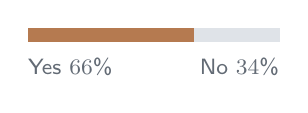
\begin{tikzpicture}[x=1cm,y=1cm]

  \pgfmathsetmacro{\BarYes}{3.2*\PolicyShare/100}
  \pgfmathsetmacro{\BarNoShare}{100-\PolicyShare}

  \fill[Employer]
    (0,0) rectangle (\BarYes,0.18);

  \fill[Rule]
    (\BarYes,0) rectangle (3.20,0.18);

  \node[
    anchor=north west,
    inner xsep=0pt,
    font=\fontsize{8.5}{10}\selectfont,
    text=Muted
  ] at (0,-0.08)
    {Yes \pgfmathprintnumber[fixed,precision=0]{\PolicyShare}\%};

  \node[
    anchor=north east,
    inner xsep=0pt,
    font=\fontsize{8.5}{10}\selectfont,
    text=Muted
  ] at (3.20,-0.08)
    {No \pgfmathprintnumber[fixed,precision=0]{\BarNoShare}\%};

\end{tikzpicture}
\par}

\end{column}

\end{columns}

\vfill

\Takeaway{
Company-wide policies are the largest single route,
alongside individual and informal arrangements.
}

\SlideNote{
Employee base: N=869; employed respondents selecting neither
``None'' nor ``Don't know'' in the original availability question.
Employer base: N=303. Samples are separate and unmatched.
}

\end{frame}

% ==========================================================
% AWARENESS
% ==========================================================

\begin{frame}[t]{TG-FWAR Awareness}

\CropPNG{\FigAwareness}
  {0.01}{0.09}{0.01}{0.11}
  {4.95cm}

\vfill

\Takeaway{
About half of each sample report familiarity;
employees are more likely to be unaware.
}

\SlideNote{
Bases: currently employed employees, N=1,004; employers, N=303.
Familiarity is self-reported. Samples are separate and unmatched.
}

\end{frame}

% ==========================================================
% REQUESTS AND OUTCOMES
% ==========================================================

\begin{frame}[t]{Requests and Outcomes}

\Subline{Formal FWA requests since TG-FWAR took effect}

\begin{columns}[T,onlytextwidth]

\begin{column}{0.48\textwidth}

\PanelTitle{Employee}{Employees}

\CropPNG{\FigRequests}
  {0.025}{0.12}{0.515}{0.23}
  {3.40cm}

\end{column}

\begin{column}{0.48\textwidth}

\PanelTitle{Employer}{Employers}

\CropPNG{\FigRequests}
  {0.525}{0.12}{0.025}{0.23}
  {3.40cm}

\end{column}

\end{columns}

\vfill

\Takeaway{
Among employees who had heard of TG-FWAR, 65.7\% applied;
64.0\% of applicants reported full approval.
}

\SlideNote{
Request questions were shown only to respondents who had heard of
TG-FWAR (employees also had to be currently employed).
Request bases: employees N=832; employers N=280.
Outcome bases: applicants N=547; receiving employers N=154.
Employee outcomes concern individual requests; employer outcomes
concern within-firm approval shares
(all or most=60--100\%; some or about half=10--59\%;
few or none=0--9\%). Samples are separate and unmatched.
}

\end{frame}

% ==========================================================
% THE CHOICE EXPERIMENT
% ==========================================================

\begin{frame}[t]{The Choice Experiment}

\begin{columns}[T,onlytextwidth]

\begin{column}{0.60\textwidth}

\PanelTitle{Navy}{An example choice}

\FitFigure{\FigDCEExample}{4.60cm}
  {Example DCE choice task}

\end{column}

\begin{column}{0.36\textwidth}

\PanelTitle{Navy}{How it works}

\setbeamerfont{itemize/enumerate body}{
  size=\fontsize{11}{14}\selectfont
}

{\begin{itemize}
  \setlength{\itemsep}{0.18cm}
  \item Two job profiles per task
  \item Six tasks per respondent
  \item Arrangements and salary vary across profiles
  \item Parallel employee and employer versions
\end{itemize}
}

\end{column}

\end{columns}

\vfill

\Takeaway{
Choices reveal trade-offs between salary and work arrangements,
so each arrangement can be valued in salary terms (WTP).
}

\end{frame}

% ==========================================================
% EMPLOYEE PREFERENCES
% ==========================================================

\begin{frame}[t]{Employee Preferences}

\FitFigure{employee_main.png}{6cm}
  {Employee FWA WTP estimates and 95\% confidence intervals}

\vfill

\Takeaway{
Among FWAs, fully remote work has the largest estimated
employee salary-equivalent value.
}

\SlideNote{
Conditional logit; N=1,020; respondent-clustered SEs, 95\% CIs.
Negative values indicate salary employees would forgo.
Bases: onsite, fixed hours, full-time, high job-loss risk,
hierarchical culture and long commute.
Fully remote includes no commute.
}

\end{frame}

% ==========================================================
% EMPLOYER PREFERENCES
% ==========================================================

\begin{frame}[t]{Employer Preferences}

\FitFigure{employer_main.png}{6cm}
  {Employer FWA WTP estimates and 95\% confidence intervals}

\vfill

\Takeaway{
Employers require the largest estimated salary offset
for fully remote work.
}

\SlideNote{
Conditional logit; N=303; respondent-clustered SEs, 95\% CIs.
Negative values indicate salary reductions required by employers.
Bases: onsite, fixed hours, full-time, low turnover and
collaborative culture.
These are hypothetical trade-offs, not wage recommendations.
}

\end{frame}

% ==========================================================
% VALUATION GAPS
% ==========================================================

\begin{frame}[t]{Valuation Gaps}

\FitFigure{wtp_gap_employee_employer.png}{6cm}
  {Employee--employer salary-adjustment gaps and 95\% CIs}

\vfill

\Takeaway{
Fully remote work and part-time work show the largest
FWA valuation gaps in point estimates.
}

\SlideNote{
Gap = employee minus employer salary adjustment;
N=1,020 and 303, respectively.
Positive gaps indicate larger employer-required reductions.
Samples are unmatched; fully remote work includes no commute
in the employee DCE.
}

\end{frame}

% ==========================================================
% EMPLOYEE HETEROGENEITY
% ==========================================================

\begin{frame}[t]{Employee Heterogeneity}

\begin{columns}[T,onlytextwidth]

\begin{column}{0.48\textwidth}

\PanelTitle{Employee}{Gender and work location}
\Subline{Male / Female}

\FitFigure{employee_gender_remote.png}{3.75cm}
  {1--2 days WFH\\
   3--4 days WFH\\
   Fully remote\\[0.15cm]
   WTP estimates and 95\% CIs}

\end{column}

\begin{column}{0.48\textwidth}

\PanelTitle{Employee}{Age and work schedules}
\Subline{19--39 / 40+}

\FitFigure{employee_age_schedule.png}{3.75cm}
  {Staggered hours\\
   Compressed 4-day week\\[0.15cm]
   WTP estimates and 95\% CIs}

\end{column}

\end{columns}

\vfill

\Takeaway{
Point estimates suggest women value remote work more;
work-schedule valuations also differ by age.
}

\SlideNote{
Conditional-logit subgroup estimates with 95\% CIs.
Men N=593; women N=424
(three respondents outside the male/female coding excluded).
Ages 19--39 N=546; 40+ N=474.
Point-estimate contrasts do not establish statistical differences.
}

\end{frame}

% ==========================================================
% CONSTRAINTS AND CONCERNS
% ==========================================================

\begin{frame}[t]{Constraints and Concerns}

\Subline{Employer WFH valuations, by subgroup}

\begin{columns}[T,onlytextwidth]

\begin{column}{0.48\textwidth}

\PanelTitle{Employer}{Physical-presence requirements}

\FitFigure{\FigPresence}{3.95cm}
  {Employer WFH valuations by physical-presence requirements}

\end{column}

\begin{column}{0.48\textwidth}

\PanelTitle{Employer}{Reported concerns}

\FitFigure{\FigConcerns}{3.95cm}
  {Employer WFH valuations by concern score}

\end{column}

\end{columns}

\vfill

\Takeaway{
Greater physical-presence needs and higher concerns
are associated with larger required WFH salary offsets.
}

\SlideNote{
Conditional logit.
Most roles require presence: N=98; some/few: N=205.
Concern score: mean of productivity, coordination and creativity
concerns; low ($\leq$3) N=93, high ($>$3) N=210.
Associations are not causal.
}

\end{frame}

% ==========================================================
% CURRENT PRACTICE AND PREFERENCES
% ==========================================================

\begin{frame}[t]{Current Practice and Preferences}

\begin{columns}[T,onlytextwidth]

\begin{column}{0.48\textwidth}

\PanelTitle{Employee}{Employees}
\Subline{Current users / Non-users}

\FitFigure{employee_current_arrangement.png}{3.75cm}
  {Compressed workweek and part-time\\[0.15cm]
   WTP by current arrangement}

\end{column}

\begin{column}{0.48\textwidth}

\PanelTitle{Employer}{Employers}
\Subline{Any current WFH / No current WFH}

\FitFigure{\FigEmployerPractice}{3.75cm}
  {Remote-work WTP by current WFH practice}

\end{column}

\end{columns}

\vfill

\Takeaway{
Current arrangements are associated with preferences,
but experience and selection cannot be separated here.
}

\SlideNote{
Employee current-use interaction model: N=1,004 currently employed
respondents; each arrangement compared with its non-users.
Employer subgroup models: any current WFH N=243; none N=60.
Current practice is self-reported.
}

\end{frame}

% ==========================================================
% KEY FINDINGS
% ==========================================================

\begin{frame}[t]{Key Findings}

\setbeamerfont{itemize/enumerate body}{
  size=\fontsize{11}{13.5}\selectfont
}

\begin{columns}[T,onlytextwidth]

\begin{column}{0.32\textwidth}

\PanelTitle{Navy}{Access and use}

{\hyphenpenalty=10000\raggedright
\begin{itemize}
  \setlength{\itemsep}{0.16cm}
  \item \PolicyShare\% of employers have a formal written FWA policy
  \item Familiar with TG-FWAR:
        55.1\% of employees; 52.8\% of employers
  \item 64.0\% of employee applicants report full approval
\end{itemize}
}

\end{column}

\begin{column}{0.32\textwidth}

\PanelTitle{Employee}{Employee side}

{\hyphenpenalty=10000\raggedright
\begin{itemize}
  \setlength{\itemsep}{0.16cm}
  \item Fully remote work has the largest FWA value
        in point estimates
  \item Point estimates vary by gender (remote work)
        and age (schedules)
\end{itemize}
}

\end{column}

\begin{column}{0.32\textwidth}

\PanelTitle{Employer}{Employer side}

{\hyphenpenalty=10000\raggedright
\begin{itemize}
  \setlength{\itemsep}{0.16cm}
  \item Largest FWA gaps: fully remote and part-time work
  \item WFH valuations vary with physical-presence requirements
        and reported concerns
\end{itemize}
}

\end{column}

\end{columns}

\vfill

\Takeaway{
Support should address both understanding of the request process
and practical implementation.
}

\end{frame}

% ==========================================================
% SUPPORTING FWA ADOPTION
% ==========================================================

\begin{frame}[t]{Supporting FWA Adoption}

\Subline{Potential responses to test, informed by the survey patterns}

\vspace{0.05cm}

{\fontsize{11}{14}\selectfont
\renewcommand{\arraystretch}{1.30}
\setlength{\tabcolsep}{6pt}

\begin{tabularx}{\textwidth}{
  @{}
  >{\RaggedRight\arraybackslash}X
  >{\RaggedRight\arraybackslash}X
  >{\RaggedRight\arraybackslash}X
  @{}
}

\toprule
{\color{Navy}\textbf{Evidence / question}} &
{\color{Navy}\textbf{Support to consider}} &
{\color{Navy}\textbf{What to test}} \\

\midrule

Incomplete familiarity with TG-FWAR &
Clear guidance and worked examples &
Understanding and request behaviour \\

\addlinespace[0.12cm]

Operational requirements and reported concerns &
Task-specific options and HR / manager support &
Feasibility, coordination and performance \\

\addlinespace[0.12cm]

Preferences vary with current practice &
Time-limited, evaluated pilots &
Learning, take-up and sustained use \\

\bottomrule

\end{tabularx}
}

\vfill

\SlideNote{
These are candidate interventions.
The survey does not establish whether preference differences
are caused by misinformation, experience or operational constraints.
}

\end{frame}

% ==========================================================
% APPENDIX
% ==========================================================

\StartAppendix

\begin{frame}[plain,noframenumbering]

\vfill
\vspace{0.25cm}

{\color{Navy}\fontsize{34}{40}\selectfont\bfseries
Appendix\par}

\vspace{0.35cm}

{\color{Muted}\fontsize{14}{19}\selectfont
Additional results, methods and supporting evidence\par}

\end{frame}

% ==========================================================
% SAMPLE AND DESCRIPTIVE DETAILS
% ==========================================================

\AppendixFigure
  {Employee Sample}
  {appendix_employee_sample.png}
  {Employee sample characteristics}

\AppendixFigure
  {Employer Sample}
  {appendix_employer_sample.png}
  {Employer sample characteristics}

\AppendixFigure
  {Question Routing}
  {appendix_routing.png}
  {Question eligibility and denominators}

\AppendixFigure
  {Availability Adjustments}
  {appendix_availability_adjustments.png}
  {Original versus adjusted availability and provision}

\AppendixFigure
  {Approval Categories}
  {appendix_approval_categories.png}
  {Original employer approval categories}

\AppendixFigure
  {Future FWA Plans}
  {appendix_fwa_plans.png}
  {Plans to expand, maintain or reduce FWAs}

% ==========================================================
% EMPLOYEE HETEROGENEITY
% ==========================================================

\AppendixFigure
  {Employee WTP: Gender}
  {employee_gender.png}
  {Full gender results}

\AppendixFigure
  {Employee WTP: Age}
  {employee_age.png}
  {Full age results}

\AppendixFigure
  {Employee WTP: Any Caregiving}
  {employee_any_caregiving.png}
  {No caregiving / Any caregiving}

\AppendixFigure
  {Employee WTP: Role}
  {employee_role.png}
  {Employee role-level results}

\AppendixFigure
  {Employee WTP: Education}
  {employee_edu.png}
  {Education-group results}

\AppendixFigure
  {Employee WTP: Availability}
  {employee_availability.png}
  {WTP by corresponding FWA availability}

\AppendixFigure
  {Employee WTP: Current Use}
  {employee_current_arrangement.png}
  {Full current-arrangement results}

% ==========================================================
% EMPLOYER HETEROGENEITY
% ==========================================================

\AppendixFigure
  {Employer WTP: Firm Size}
  {employer_size.png}
  {Organisation-size results}

\AppendixFigure
  {Employer WTP: Respondent Role}
  {employer_role.png}
  {Respondent-role results}

\AppendixFigure
  {Industry: Work Location}
  {employer_industry_place.png}
  {Industry-specific location preferences}

\AppendixFigure
  {Industry: Work Schedule}
  {employer_industry_time.png}
  {Industry-specific schedule preferences}

\AppendixFigure
  {Industry: Workload}
  {employer_industry_load.png}
  {Industry-specific workload preferences}

\AppendixFigure
  {Industry: Turnover}
  {employer_industry_turnover.png}
  {Industry-specific turnover preferences}

\AppendixFigure
  {Industry: Work Culture}
  {employer_industry_culture.png}
  {Industry-specific work-culture preferences}

\AppendixFigure
  {Productivity Concerns}
  {employer_concern_productivity.png}
  {Employer productivity concerns}

\AppendixFigure
  {Coordination Concerns}
  {employer_concern_coordination.png}
  {Employer coordination concerns}

\AppendixFigure
  {Creativity Concerns}
  {employer_concern_creativity.png}
  {Employer creativity and innovation concerns}

\AppendixFigure
  {Technological Readiness}
  {employer_tech_readiness.png}
  {Employer technological readiness}

\AppendixFigure
  {Salary-Reduction Beliefs}
  {employer_salary_belief.png}
  {Employer salary-reduction beliefs}

% ==========================================================
% METHODS AND ROBUSTNESS
% ==========================================================

\AppendixFigure
  {DCE Design}
  {appendix_dce_design.png}
  {Attributes, levels and reference categories}

\AppendixFigure
  {WTP Interpretation}
  {appendix_wtp_definition.png}
  {WTP calculation and sign conventions}

\AppendixFigure
  {Conditional Logit Estimates}
  {appendix_conditional_logit.png}
  {Coefficients and standard errors}

\AppendixFigure
  {Response Patterns}
  {appendix_response_patterns.png}
  {Choice-position and same-side response patterns}

\AppendixFigure
  {Response-Quality Checks}
  {employee_same_side.png}
  {Estimates excluding same-side respondents}

\AppendixFigure
  {Salary Sensitivity}
  {employee_salary_trim.png}
  {Salary-trimming robustness}

\AppendixFigure
  {Choices and Relative Salary}
  {employee_dominance_robust_1.png}
  {Choice patterns under the specified attribute-ordering assumptions}

\AppendixFigure
  {Stated and Observed Trade-offs}
  {employee_dce_hedonic.png}
  {DCE WTP and adjusted observed salary differentials}

% ==========================================================
% RELATED LITERATURE
% ==========================================================

\begin{frame}[t]{Related literature}

\end{frame}

\end{document}
